\section{Theory}

\begin{frame}{The sand-moving problem}
    \footnotesize
    A child wants to make a pile of sand in the shape of a castle.

    \textbf{Cost:} 1 kcal per shovel and per meter horizontally.

    \textbf{Target:} Minimize the total cost.

    \begin{figure}
        \captionsetup{font=scriptsize}
        \centering
        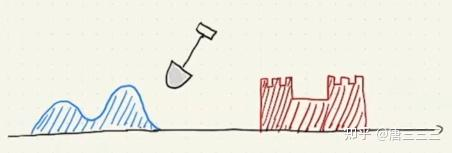
\includegraphics[width=0.8\textwidth]{png/SandMoving.jpg}
        \caption{The sand-moving problem.}
    \end{figure}

    \pause
    Let's denote the source shape by $f(x)$ and the target by $g(x)$. 
    The sand-moving problem cound be formulated as: 
    find a \textbf{transport mapping} $T:\R\to\R$ to minimize
    \begin{equation}
        \int_{\R} |T(x)-x|f(x)\;dx,
    \end{equation}
    which satisfies
    \begin{equation}
        \int_{T(U)} g(x)\;dx = \int_{U} f(x)\;dx\; \text{for all open interval}\; U\subset\R.
    \end{equation}
\end{frame}

\begin{frame}{The allocation problem}
    \footnotesize
    There are some steel coils to be transported from warehouses to factories.
    The transport cost is \$1 per coil and per kilometer.
    How to minimize the total cost?

    \begin{figure}
        \captionsetup{font=scriptsize}
        \centering
        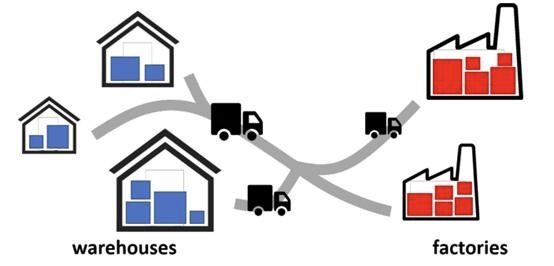
\includegraphics[width=0.6\textwidth]{png/SteelTransport.jpg}
        \caption{The allocation problem.}
    \end{figure}

    \pause\vspace{-.5em}
    Assume the $i$-th warehouse has $a_i$ coils and the $j$-th factory
    needs $b_i$ coils. And assume the distance between the $i$-th warehouse
    and the $j$-th factory is $d_{ij}$. The allocation problem could be 
    formulated as: find a \textbf{transport matrix} $v_{ij}$ to minimize
    \begin{equation}
        \sum_{i,j} d_{ij}v_{ij}
    \end{equation}
    which satisfies
    \begin{equation}
        a_i=\sum_{j} v_{ij},\quad \forall i,
        \qquad \text{and} \qquad 
        b_j=\sum_{i} v_{ij},\quad \forall j.
    \end{equation}
\end{frame}

\begin{frame}{The Kantorovich formulation}
    \footnotesize
    To give an general formulation of OT, 
    we first recall the three main scenarios for OT.

    \begin{figure}
        \captionsetup{font=scriptsize}
        \centering
        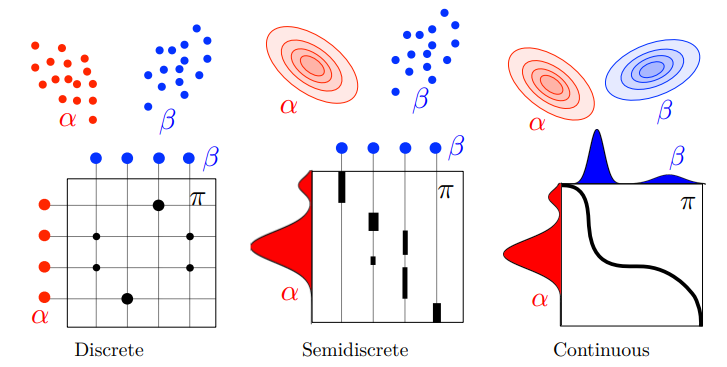
\includegraphics[width=0.6\textwidth]{png/3TypesOfOT.png}
    \end{figure}

    \pause
    Given two probability measures $\mu$ on $\mX$ and $\nu$ on $\mY$, and a 
    cost function $c(x,y)$. 
    The Kantorovich formulation\footfullcite{Kantorovich1942} of OT is 
    \begin{equation}
        \mL_c(\mu,\nu)=\min_\pi \; \int_{\mX\times \mY} c(x,y) \;d\pi(x,y),
    \end{equation}
    where $\pi$ is a measure on $\mX\times \mY$, whose
    marginals are $\mu$ and $\nu$, that is,
    \begin{equation}
        \mu = \int_{\mY} \pi(\cdot, y) \;dy,\qquad 
        \nu = \int_{\mX} \pi(x, \cdot) \;dx.
    \end{equation}
\end{frame}

\begin{frame}{Metric properties of OT}
    \footnotesize
    Here we assume $\mX=\mY$ and $c(x,y)=d(x,y)^p\;(p>1)$, where $d$ is a distance on $\mX$.
    Denote $\pbms$ the set of probability measures on $\mX$.

    \pause
    \begin{Thm}[Wasserstein distance]
        Under the above assumptions, $\mL_c(\mu,\nu)^{1/p}$ is a distance on $\pbms$.
    \end{Thm}

    The distance $\wass_p(\mu,\nu):=\mL_c(\mu,\nu)^{1/p}$ is called $p$-Wasserstein distance.

    \pause

    \begin{Def}[Weak convergence]
        Assume $\mX$ is compact. Say $(\mu_k)_{k\geq 1}\subset \pbms$ converges
        weakly to $\mu\in\pbms$ if
        \begin{equation}
            \int_{\mX} g\;d\mu_k \to \int_{\mX}g\;d\mu,\quad \forall g\in\cfun.
        \end{equation}
    \end{Def}

    \begin{Thm}[Wasserstein distance and weak convergence\footfullcite{Villani2009}]
        On a compact domain $\mX$, $(\mu_k)_{k\geq 1}\subset \pbms$ converges 
        weakly to $\mu\in\pbms$ if and only if $\wass_p(\mu_k,\nu)\to 0$.
    \end{Thm}
\end{frame}